% !TEX root = ../main.tex

\chapter{Paper reproduction}
\label{ch:paper_reproduction}
This chapter relies on the article "Computer-Aided Diagnosis of Prostate Cancer Using a Deep Convolutional Neural Network from Multiparametric MRI" from Song et al.\cite{07}, shortly presented in chapter \ref{ch:literature_review}. It aims at reproducing the experiment of the paper in order to acquire the medical, theoretical and technical background before proposing a transfer learning method as a way to improve the classification using other body parts, which overcome the lack of available data (see chapter \ref{ch:transfer_learning}).\\
Song et al. \cite{07} proposed a deep convolutional neural network (DCNN) method to detect prostate cancer based on the SPIE-AAPM-NCI PROSTATEx Challenge dataset. This dataset is one of the biggest available dataset for prostate cancer classification. The two different output classes of the latter are benign lesion (class 0) and malignant lesion (class 1). This paper explains all the steps to follow with the goal of building a computer-aided-diagnosis (CAD) system for prostate cancer detection. Moreover, it also provides results about the algorithm performance, which can be used as a benchmark to compare with the results of the reproduction of the experiment. However, since the article gives no information about the results their model got on the official PROSTATEx challenge test set, the reproduction of the experiment will fill that gap.\\
This chapter is built top-down: first a superficial overview of the entire process is established in order to understand the purpose of the experiment as a whole. Then, each part or theoretical notion of the experiment is deeply described. The structure of the dataset is detailed, all steps of its processing are explained and the techniques used as verification of the proper functioning of the algorithm are presented. After the processing of the data, the training phase is deepened and all hyperparameters, options and implementation choices are given to ensure the reproductibility of the experiment. This part is followed by the presentation of the raw results, which is itself followed by their analysis in the "discussion" section.

\section{Process overview}
Schematically, the entire experiment process can be represented as shown in figure \ref{fig:paper_reproduction_process}. The PROSTATEx dataset is composed of samples whose clinical significance is provided (labeled data) and samples without this information (unlabeled data). The latter are used for the challenge, which consists in predicting the probability of patients lesions to be malignant (class 1) or benign (class 0). In both cases, the data is processed before been used (see \ref{prostatex_data_processing} for details). After the processing, the labeled data are split into training, validation and test sets using respectively 80\%, 10\% and 10\% of all available data for each set. The training set is then given in batches as input to the neural network, which update its weight consequently. At the end of each epoch, the current model is tested on the validation set (that the model has never seen previously) and the metrics are plotted on Tensorboard (see \ref{paper_tensorboard}). If the current model has a bigger AUC and a bigger accuracy than the previous best model, it becomes the best model and it is saved.  When the training phase reaches the defined number of epochs, the model is then tested on the test set. This same model is also used to take part in the PROSTATEx challenge to output predictions into a .csv file for each patient and findings.

\begin{figure}[!h]
\centering
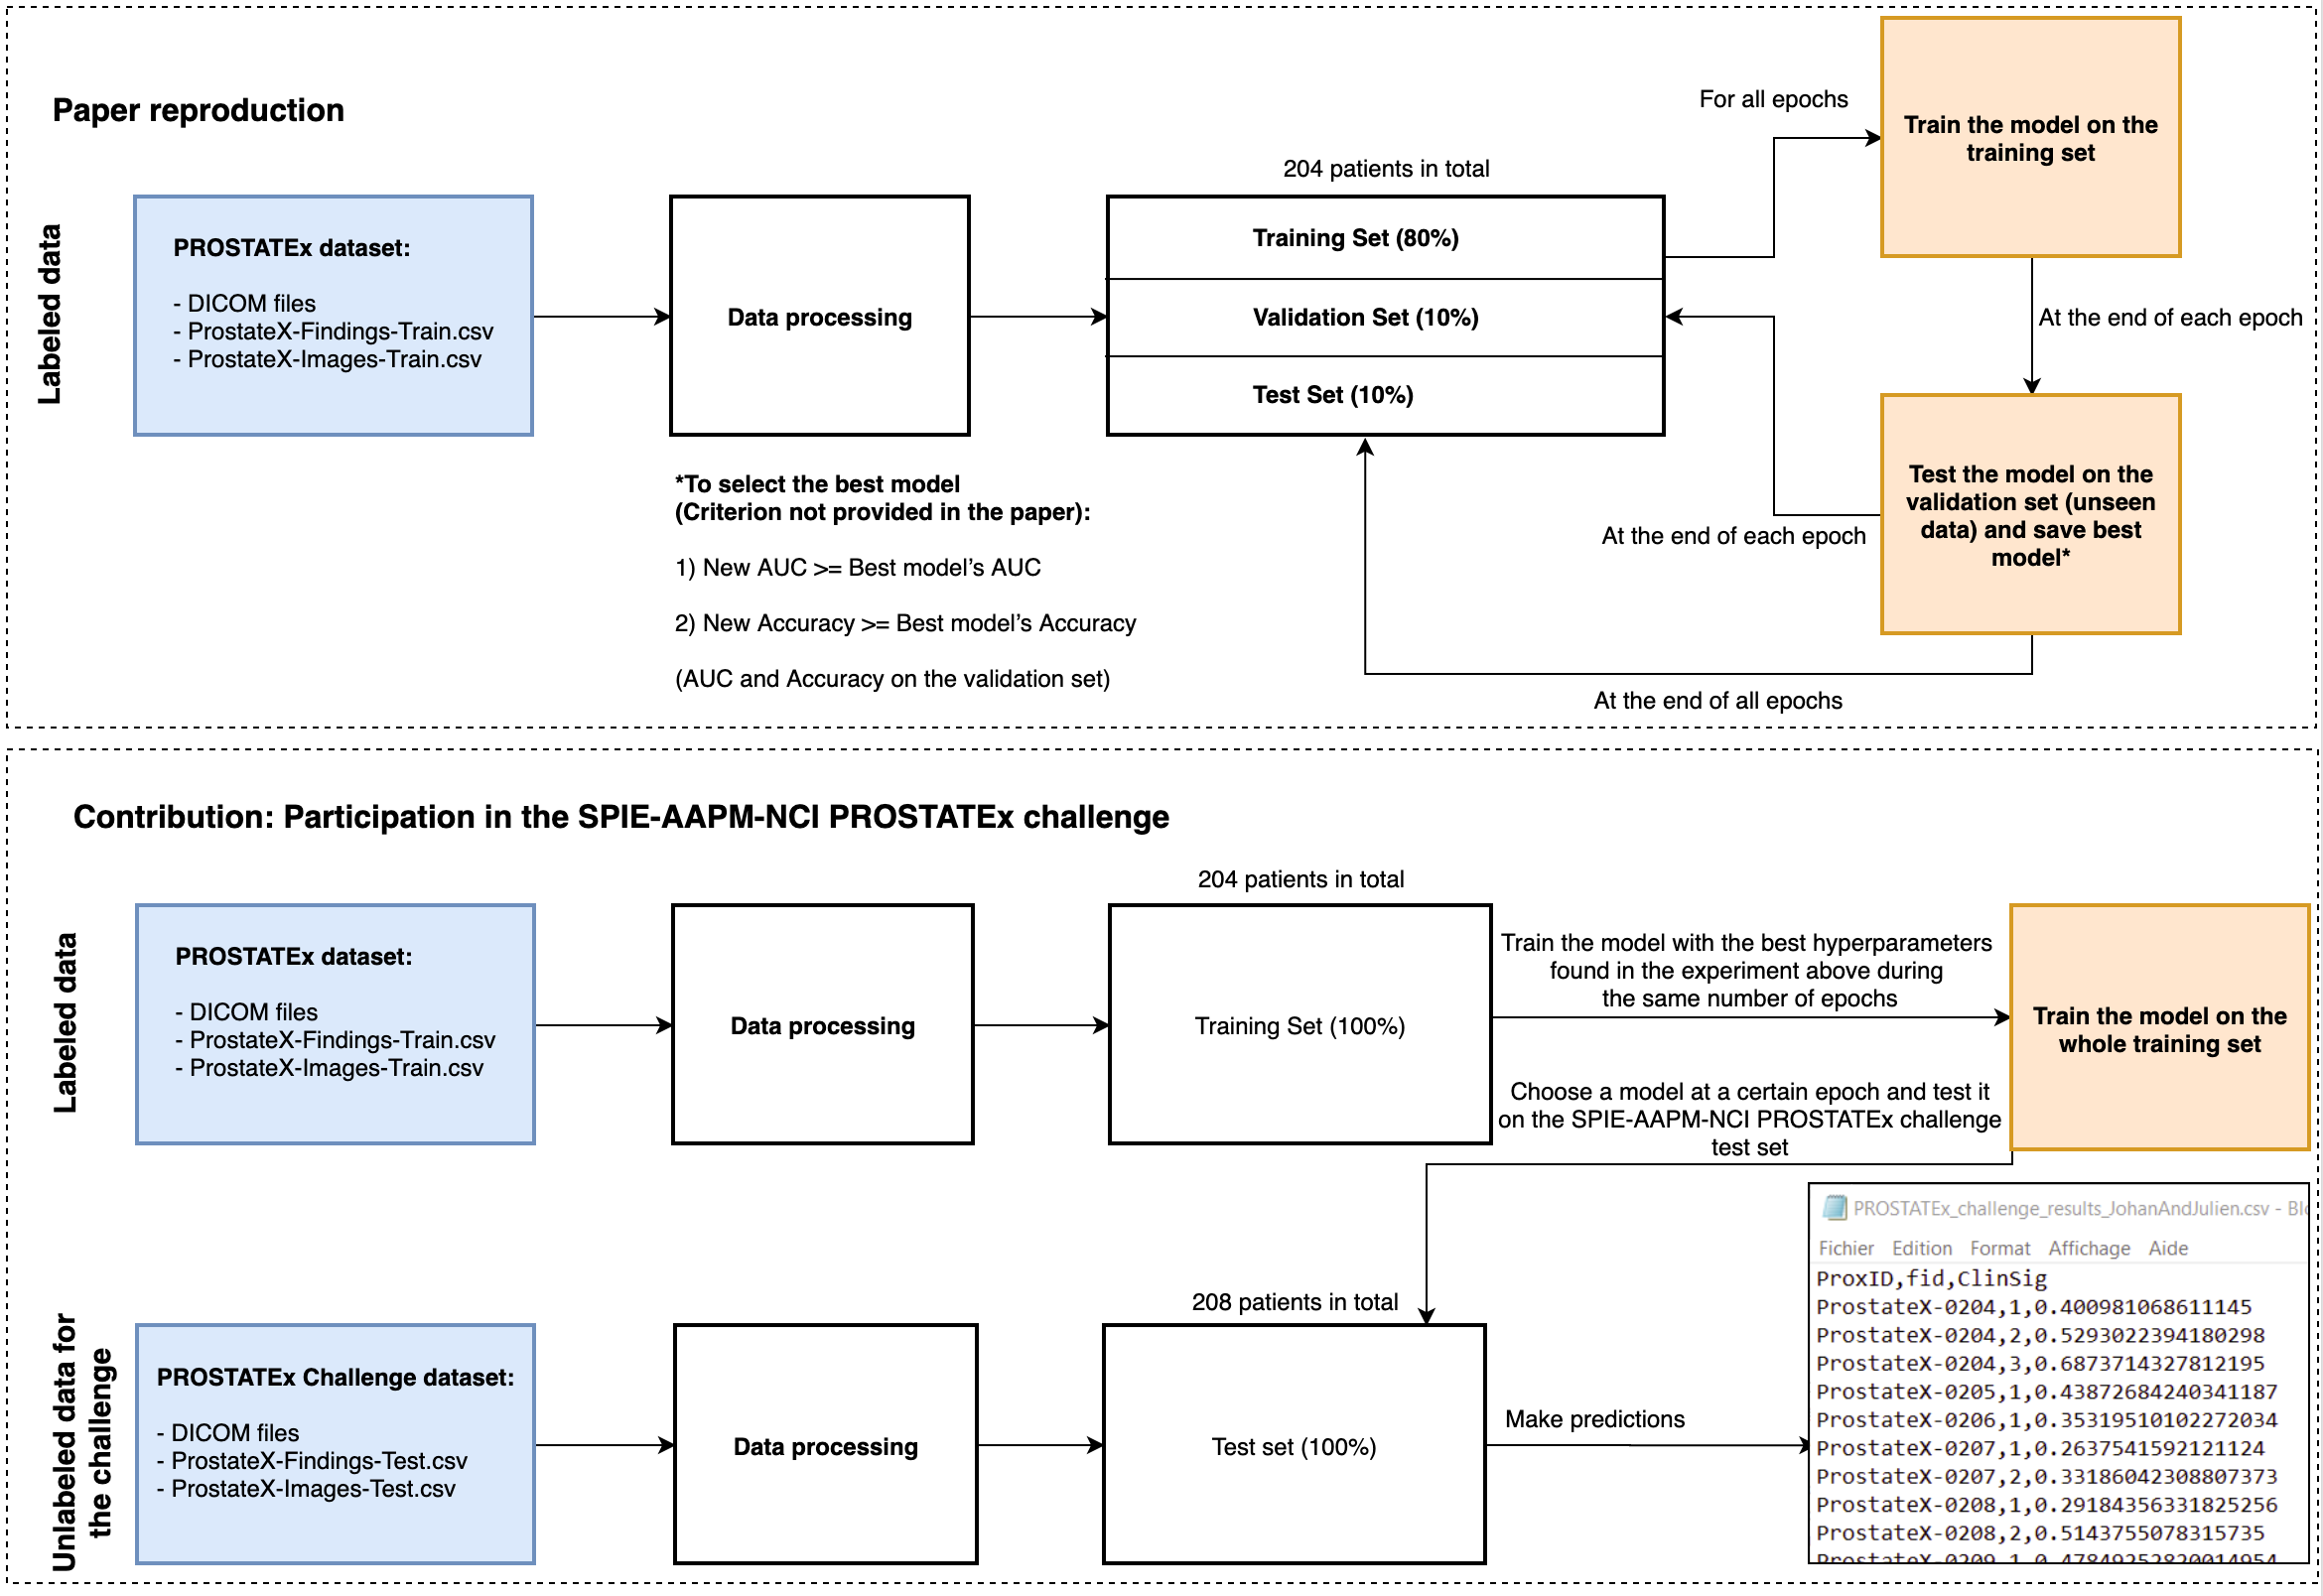
\includegraphics[width=1\textwidth, keepaspectratio=true]{./figures/paper_reproduction_process.png}
\caption{Paper reproduction experiment}
\label{fig:paper_reproduction_process}
\end{figure}


\section{PROSTATEx: Data processing}
\label{prostatex_data_processing}
\subsection{Dataset description}
\label{prostatex_dataset_description}
\subsection{From DICOM to NumPy arrays}
\subsection{From NumPy arrays to augmented stacked images}
\subsection{From NumPy arrays to augmented non-stacked images}
\subsection{Data processing verification}
\subsubsection{Cropping verification using red dots}
\subsubsection{Alignment visualization}

\section{Training the neural network}
\subsection{Architecture}
The model architecture used in the paper is a modified version of the VGG network from the Oxford's Visual Geometry Group (VGG). This model was initially designed as part of the Large Scale Visual Recognition Challenge 2014 that used the ImageNet dataset of 14 millions images belonging to 1000 classes. The figure \ref{fig:paper_model} illustrates its structure and its corresponding implementation in Python with the PyTorch Framework.\\
It is first composed by three convolution-dropout-max-pooling blocks followed by three fully connected-dropout blocks. Each convolutional box (in blue) in the figure represents in reality three layers: the convolutional layer, the batch normalization layer and the exponential linear unit activation function. The same principle is used for the fully connected layer box (in orange) that is divided into a fully connected layer followed by the exponential linear unit. The last fully connected box (in purple) has the same structure except that the exponential linear unit is replaced by a softmax  function for classification.\\
In comparison to the original VGG, this model keeps the small filter size of 3x3 or 1x1,  also doubles the number of filters after each convolution-dropout-max-pooling block and has a stride of 1 for all convolutions. It differs from the traditional VGG in that it makes use of a smaller number of layer since the task is simpler than the original one, it uses exponential linear units instead of rectified linear units as activation functions and adds dropout and batch normalization layers.
\begin{figure}[!h]
\centering
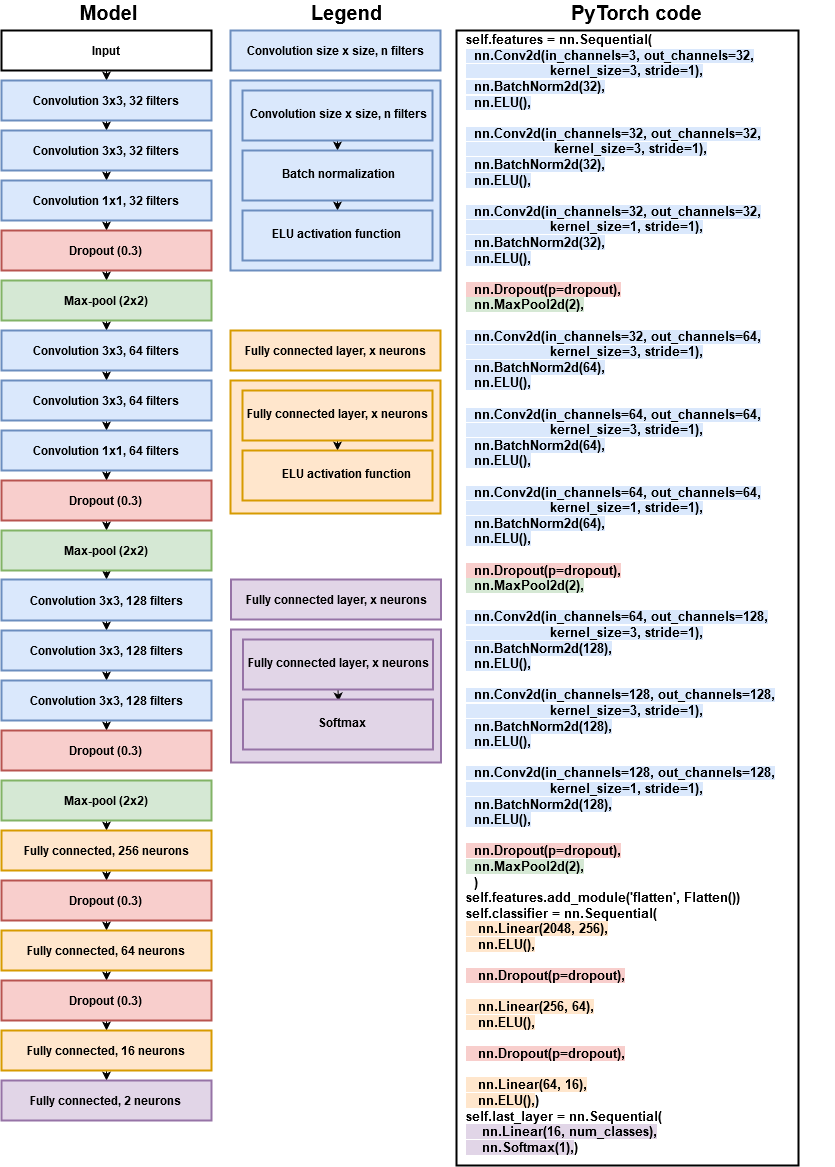
\includegraphics[width=1\textwidth, keepaspectratio=true]{./figures/model_paper_manual.png}
\caption{Model architecture with the corresponding PyTorch code}
\label{fig:paper_model}
\end{figure}
\subsection{Criterion to save the best model}
\subsection{Tensorboard}
During the experiment the following metrics are registered: loss, accuracy, precision, recall, F1-score, specificity and AUC. These metrics are computed separately on the training and on the validation sets at the end of each epoch. They are then stored across all epochs and plotted on the same figure thanks to Tensorboard at the end of the process. Subsequently, this is also the case for the metrics measured on the test set.\\
"Tensorboard provides the visualization and tooling needed for machine learning experimentation:
\begin{itemize}
\item Tracking and visualizing metrics.
\item Visualizing the model graph (ops and layers).
\item Viewing histograms of weights, biases, or other tensors as they change over time.
\item Projecting embeddings to a lower dimensional space.
\item Displaying images, text, and audio data"\cite{39}.
\end{itemize}
In this experiment, Tensorboard is mainly used to plot the Matplotlib figures of the model performance. In addition to this, written reports regarding which model was the best and the results it reached are also added on the dashboard.
\label{paper_tensorboard}
\subsection{Script options}
\subsection{Experimental setup}
\subsection{Training verification}
\subsubsection{Gradient flow visualization}

\section{Results}

\section{Discussion}